\documentclass[12pt,oneside]{report}
\usepackage{listings}
\usepackage[T1]{fontenc}		
\usepackage[utf8x]{inputenc}
\usepackage[ngerman]{babel}

\usepackage{parskip}			

\usepackage[a4paper,		
	    left=2.5cm,				
	    right=2.5cm,			
	    top=1.5cm,				
	    bottom=1.5cm,			
	    marginparsep=5mm,		
	    marginparwidth=10mm, 	
	    headheight=7mm,			
	    headsep=1.2cm,			
	    footskip=1.5cm,			
	    includeheadfoot]{geometry}

\usepackage{fancyhdr}						
\pagestyle{fancy}							
\fancyhf{}									
\setlength{\headwidth}{\textwidth}			
\fancyfoot[R]{\thepage} 					
\fancyfoot[L]{\leftmark}					
\fancyhead[R]{\IhreArbeit}					
\fancyhead[L]{\IhrVorname\ \IhrNachname}	
\renewcommand{\chaptermark}[1]{			
  \markboth{Kapitel \thechapter. #1}{}}
\renewcommand{\headrulewidth}{0.5pt}		
\renewcommand{\footrulewidth}{0.5pt}		
\fancypagestyle{plain}{					
  \fancyhf{}								
  \fancyfoot[C]{\thepage}					
  \fancyhead[R]{\IhreArbeit}				
  \fancyhead[L]{\IhrVorname\ \IhrNachname}	
}

\usepackage{amsmath}			
\usepackage{amssymb}
\usepackage[intlimits]{empheq}

\usepackage[sc]{mathpazo}		
\usepackage{pifont}				

\usepackage[format=hang,		
            font={footnotesize},
            labelfont={bf},
            margin=1cm,
            aboveskip=5pt,
            position=bottom]{caption}

\usepackage{graphicx}							
\usepackage[svgnames,table,hyperref]{xcolor} 
\usepackage{tikz}								
\usetikzlibrary{positioning,arrows,plotmarks} 

\usepackage{microtype,relsize}			
\newcommand*{\Sperren}[1]{\textls*[100]{#1}}

\usepackage{xurl}
\usepackage[table]{xcolor}
\usepackage{multirow}
\usepackage{nicematrix}
\usepackage{hhline}
\usepackage{ifthen}
\usepackage{subfig}
\usepackage{tabularray}

\usepackage{listings}			% Darstellung von Quellcode
\definecolor{gray}{rgb}{0.5, 0.5, 0.5}
\definecolor{blue}{rgb}{0.0, 0.0, 1.0}
\definecolor{darkgreen}{rgb}{0.0, 0.2, 0.13}
\definecolor{mauve}{rgb}{0.88, 0.69, 1.0}
\lstset{frame=tb,
	language=Java, 
	aboveskip=3mm,
	belowskip=3mm,
	showstringspaces=false,
	columns=flexible,
	basicstyle={\small\ttfamily},
	numbers=left,
	%	numberstyle=\tiny\color{gray},
	%	keywordstyle=\color{blue},
	%	commentstyle=\color{dkgreen},
	%	stringstyle=\color{mauve},
	breaklines=true,
	breakatwhitespace=true,
	tabsize=3,
	mathescape=false}


\newcommand*{\IhrVorname}{Annika}
\newcommand*{\IhrNachname}{Stadelmann}
\newcommand*{\IhrStudiengang}{Medieninformatik}
\newcommand*{\IhreArbeit}{Studienarbeit App-Programmierung WiSe 2022/23}
\newcommand*{\IhrTitelDE}{Entwicklung eines Parkleitsystems}
\newcommand*{\IhrBearbeitungszeitraumVON}{22. November 2022}
\newcommand*{\IhrBearbeitungszeitraumBIS}{17. Januar 2023}


\usepackage[bookmarks, raiselinks, pageanchor,
            hyperindex, colorlinks,
            citecolor=black, linkcolor=black,
            urlcolor=black, filecolor=black,
            menucolor=black]{hyperref}
\hypersetup{pdftitle={\IhrTitelDE},
            pdfauthor={\IhrVorname\ \IhrNachname},
            pdfsubject={\IhreArbeit}}

\lstset{numbers=left, numberstyle=\tiny, numbersep=5pt}
\lstset{language=Java}
\usepackage{xurl}
\usepackage{subfig}
\graphicspath{ {./pictures/} }



\begin{document}
  \pagenumbering{roman}
  \begin{titlepage}					
    \thispagestyle{empty}
    \begin{center}
      \Large
      Ostbayerische Technische Hochschule Amberg-Weiden\\
      Fakultät Elektrotechnik, Medien und Informatik\\[1cm]
      Studiengang \IhrStudiengang\\[1cm]
      \textbf{\IhreArbeit}\\[1cm]
      von\\[1cm]
      \IhrVorname\ \Sperren{\textbf{\IhrNachname}}\\[1cm]
      \textbf{\IhrTitelDE}\\[1cm]
    \end{center}
    \vspace*{11cm}
    \begin{tabbing}
      \underbar{Bearbeitungszeitraum:}\qquad\= von\qquad\=\IhrBearbeitungszeitraumVON\\
                                        \> bis      \>\IhrBearbeitungszeitraumBIS
    \end{tabbing}
  \end{titlepage}
  
  \tableofcontents
  \newpage
  
  \pagenumbering{arabic}
  \chapter{Einleitung}

Im Rahmen der Studienarbeit sollte eine App als Parkleitsystem für die neun Parkhäuser um den Altstadtring in Amberg entwickelt werden. Neben der Anzeige der Parkflächen auf einer Karte, war es wichtig, auch detaillierte Informationen anzuzeigen. Dabei handelte es sich um Kosten pro Stunde, den Namen des Parkhauses oder Parkplatzes, die Anzahl der verfügbaren, belegten oder gesamten Parkplätze, sowie ein aufsteigender, gleichbleibender oder fallender Trend. Des Weiteren muss dem Nutzer auch mitgeteilt werden, ob und wann das Parkhaus geöffnet ist und ob es überhaupt befahren werden kann.

Neben der Anzeige der Daten sollte es auch die Möglichkeit geben, eine Navigation zur Parkmöglichkeit zu starten, sobald der Nutzer sich in einem bestimmten Radius um die Örtlichkeit befindet. Wenn das sogenannte Geofence betreten wird, soll neben der Navigationsmöglichkeit als Toast auch noch Text als Sprachausgabe ausgegeben werden, um den Nutzer darauf hinzuweisen, welches Parkhaus am nächsten ist und befahren werden könnte. Damit der Nutzer nun nicht durch unpassende Sprachausgabe in unangenehme Situationen gebracht wird, sollte die Möglichkeit gegeben sein, den Ton auszuschalten. Außerdem sollen die Parkmöglichkeiten auch als Liste angezeigt und favorisiert werden können.

Um die aktuellen Parkhausdaten zu bekommen, soll eine API verwendet werden, welche die Daten bereitstellt und regelmäßig aktualisiert. Die Daten sind im XML-Format und hier zu finden: \url{https://parken.amberg.de/wp-content/uploads/pls/pls.xml}

Im Folgenden Verlauf dieses Dokuments werden zunächst die verwendeten Technologien beschrieben. Anschließend werden die Vorüberlegungen zur Architektur dargelegt und die darauf folgende Implementierung vorgestellt. Im Anschluss daran findet sich eine Beschreibung, welche zeigt, wie das Projekt zu starten ist.
  \chapter{Architektur}

Die App sollte mit dem JavaScript-Framework react-native programmiert werden. Dieses Framework kann eingesetzt werden, wenn die App sowohl auf mobilen Android-, als auch ios-Geräten funktionieren soll. So kann einmal Code geschrieben werden, welche für beide Plattformen verwendet werden kann. Als Programmiersprache wird TypeScript eingesetzt. TypeScript ist wie JavaScript, nur mit Typensicherheit. So können keine Verwirrungen bezüglich des Typs einer Variable aufkommen. Zusammen mit TypeScript und dem Framework react-native wird zusätzlich noch Expo genutzt. Expo ist ein Framework, welches Werkzeuge zur Unterstützung der Entwicklung einer react-native-App bietet. 

\section{Mockups und Komponenten}
Um die Anforderungen nicht völlig durcheinander in Quell-Code zu pressen, wurden vorher Prototypen gezeichnet, welche das Design der App darstellen sollen. Dies schafft Struktur und ermöglicht es, systematisch vorzugehen. Ziel der Mockups war es, ein Design zu schaffen, welches möglichst einfach und verständlich alle relevanten Informationen auf einen Blick zeigt und es dem Nutzer ermöglicht, sich ebenfalls weitere Details anzeigen zu lassen, wenn dies gewünscht ist. Anhand dieser Mockups gelang es nun, Komponenten herauszuarbeiten, welche anschließend in Quell-Code umgewandelt werden sollten.

Da die Implementierung mit react-native erfolgt und statt Klassen Komponenten für die Benutzeroberfläche verwendet werden, wurden die Mockups in Komponenten geteilt. Die Komponente, welche alle anderen beinhalten soll, ist die ,App'. Hier findet sich auch der Button oben rechts, der in \autoref{fig:mockupApp}(a) zu sehen ist. Eine weitere Komponente bildet die Karte, welche sich über den größten Teil des Bildschirms erstreckt. Klickt man auf einen Marker, der eine Parkmöglichkeit anzeigt, so öffnet man die Komponente der Beschreibung. Diese ist beispielsweise in \autoref{fig:mockupBeschreibung}(b) zu sehen. Hier sollen Kacheln angezeigt werden, welche die einzelnen Informationen liefern. Außerdem soll hier auch der Button angezeigt werden, welcher die Navigation startet. 

\begin{figure}[h!]
	\centering
	\subfloat[\centering Dieser Entwurf zeigt die Komponente ,App' mit dem einem Button oben rechts in der Ecke. Außerdem befindet sich hier auch die Komponente mit der Karte.]{{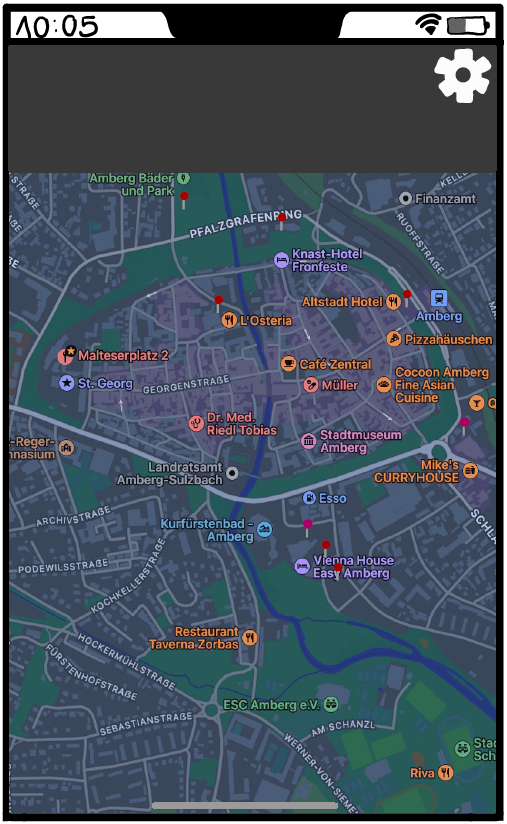
\includegraphics[width=0.45\linewidth]{mockup_app.png}}}
	\qquad
	\subfloat[\centering Zusätzlich zur Karten-Kompnente in der ,App' sieht man hier auch noch die Komponente der Beschreibung, welche sich beim Klick auf eine Parkmöglichkeit in der Karte öffnen soll. Die Kacheln zeigen die relevanten Informationen an.]{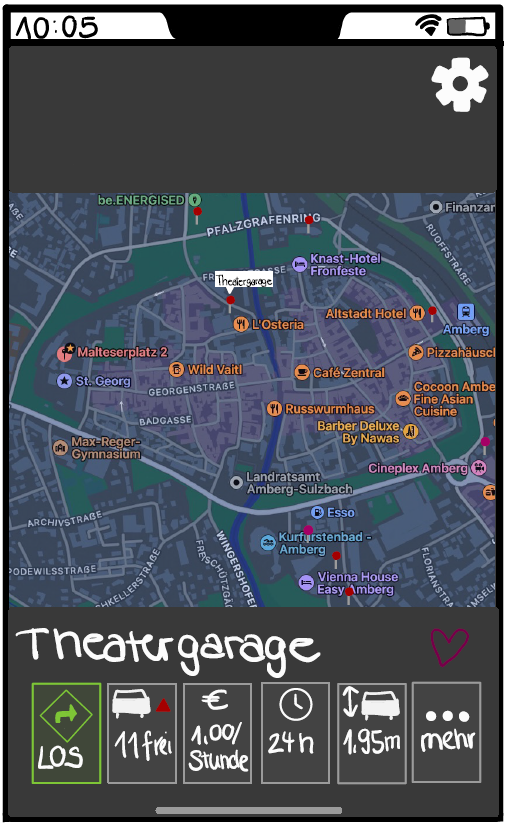
\includegraphics[width=0.45\linewidth]{mockup_beschreibung.png}}
	\caption[Diese beiden Entwürfe zeigen jeweils die ,App'-Komponente und die darin befindliche Karten-Komponente. In der rechten Abbildung öffnet man zusätzlich die Beschreibung-Komponente, welche die Karte verkleinert.]{Diese beiden Entwürfe zeigen jeweils die ,App'-Komponente und die darin befindliche Karten-Komponente. In der rechten Abbildung öffnet man zusätzlich die Beschreibung-Komponente, welche die Karte verkleinert. (Quelle: Eigens gezeichnete Mockups)}
	\label{fig:mockupApp}
	\label{fig:mockupBeschreibung}
\end{figure}

Klickt man auf das Zahnrad in \autoref{fig:mockupApp}(a) in der Komponente ,App', so soll sich eine Komponente mit den Einstellungen, wie in \autoref{fig:mockupSettings}(a) zu sehen, öffnen, in welcher der Ton an- und ausgeschaltet werden kann oder auch die Parkmöglichkeiten als Liste angezeigt werden können. Um die Parkmöglichkeiten als Liste zu sehen, wird eine weitere Komponente benötigt, wie sie in \autoref{fig:mockupParkingList}(b) erkennbar ist. Die Elemente der Liste werden mit den Favoriten zuerst nach dem Alphabet sortiert. 

\begin{figure}[h!]
	\centering
	\subfloat[\centering Die Komponente, welche das Einstellungsmenü beinhaltet. Ein Klick auf den Ton schaltet diesen entweder ein oder aus. Die Kachel darunter zeigt bei einem Klick die Parkmöglichkeiten als Liste an.]{{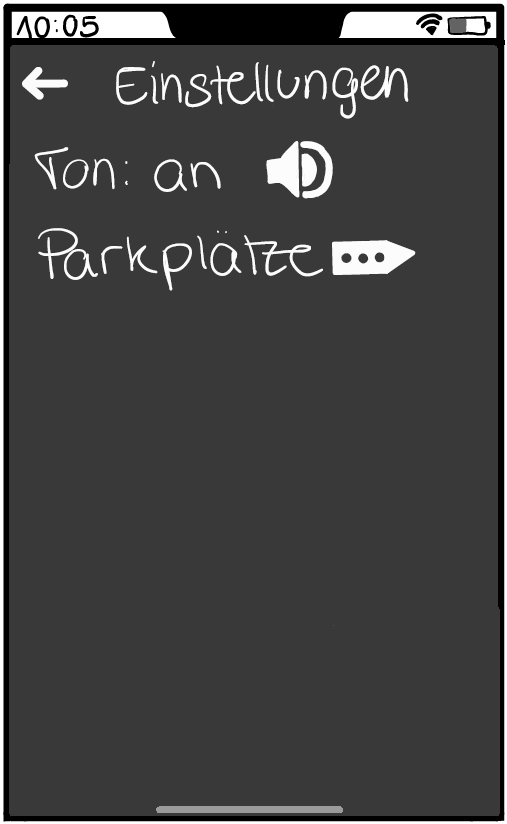
\includegraphics[width=0.45\linewidth]{mockup_settings.png}}}
	\qquad
	\subfloat[\centering Hier befindet sich die Liste der Parkhäuser, welche alphabetisch sortiert ist. Die Favoriten findet man hier ganz oben.]{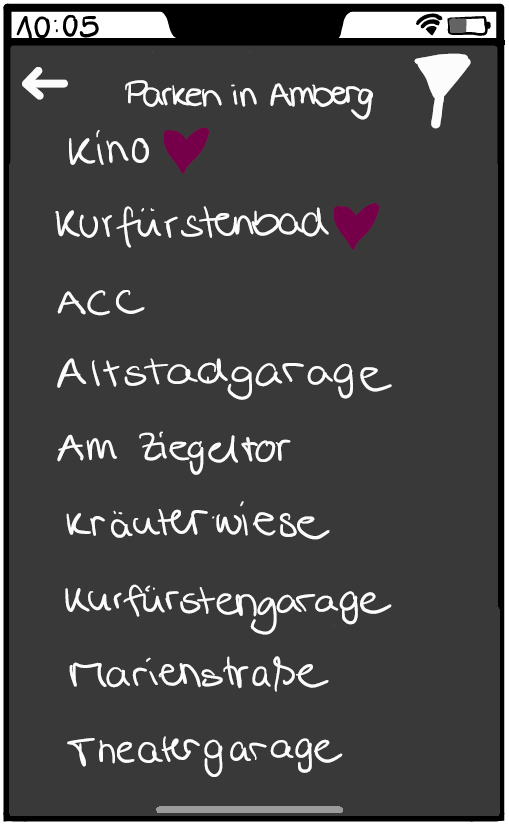
\includegraphics[width=0.45\linewidth]{mockup_parkinglist.png}}
	\caption[Auf den Entwürfen ist links das Einstellungsmenü zu sehen. Klickt man auf ,Parkplätze' oder in der Beschreibung-Komponente auf ,mehr' so gelangt man zur Ansicht der Details einer Parkmöglichkeit, was auf der rechten Seite zu sehen ist.]{Auf den Entwürfen ist links das Einstellungsmenü zu sehen. Klickt man auf ,Parkplätze' oder in der Beschreibung-Komponente auf ,mehr' so gelangt man zur Ansicht der Details einer Parkmöglichkeit, was auf der rechten Seite zu sehen ist. (Quelle: Eigens gezeichnete Mockups)}
\label{fig:mockupSettings}
\label{fig:mockupParkingList}
\end{figure}
\newpage
Klickt man in der Liste auf eine Parkmöglichkeit oder in der Beschreibung einer einzelnen auf die Kachel mit der Beschriftung "mehr", soll man auf eine Detailansicht kommen, welche alle vorhandenen Informationen des Parkhauses anzeigt. Zu sehen ist dies in \autoref{fig:mockupParkingDetails} Diese Übersicht bildet die letzte Komponente. 

\begin{figure}[h!]
	\centering
	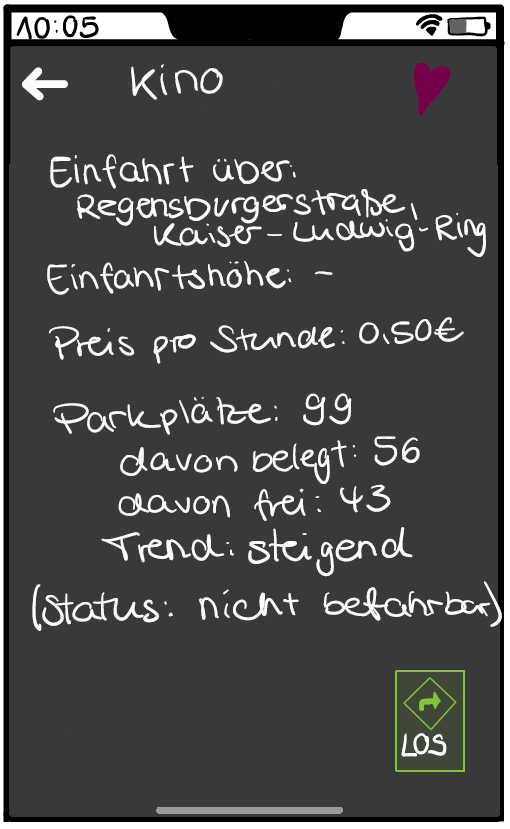
\includegraphics[width=0.45\linewidth]{mockup_parkingdetais.png}
	\caption[Diese Komponente bildet die Detailsansicht der jeweiligen Parkmöglichkeit. Zu erreichen ist diese über die Beschreibung- oder die Einstellung-Komponente.]
	{Diese Komponente bildet die Detailsansicht der jeweiligen Parkmöglichkeit. Zu erreichen ist diese über die Beschreibung- oder die Einstellung-Komponente. (Quelle: Eigens erstellte Übersicht.)}
	\label{fig:mockupParkingDetails}
\end{figure}
\newpage
In Summe sind also zunächst fünf Komponenten geplant, welche in der Komponente ,App' zu finden sind. Ob dies tatsächlich so umsetzbar ist, wird sich in der Implementierung zeigen.

\section{Datenbank}
Um die Daten nun auch sauber vom Code zu trennen, müssen Datenbanktabellen angelegt werden. Die erste Tabelle ,parkingarea' wird mit den Daten der Parkmöglichkeiten gefüllt. Hierzu bekommt jedes der neun Parkmöglichkeiten eine ID zur Identifikation. Weitere Spalten in der Tabelle beinhalten:
\begin{description}
	\item Name \\ Der Name des Parkhauses oder Parkplatzes.
	\item Adresse \\ Die Straße oder mehrere Straßen, über die die Parkmöglichkeit angefahren werden kann.
	\item Öffnungszeiten \\ Wie lange die jeweilige Parkmöglichkeit geöffnet hat.
	\item Preis pro Stunde \\ Wie viel man pro Stunde bezahlen muss, um sein Fahrzeug zu parken.
	\item Einfahrtshöhe \\ Wie hoch das Fahrzeug maximal sein darf, um in das Parkhaus zu fahren. Im vorliegenden Fall gibt es auch Parkplätze ohne maximale Einfahrtshöhe.
	\item Favorit \\ Dieser Wert gibt an, ob es sich um eine favorisiertes Parkmöglichkeit handelt oder nicht. In dem Fall gibt der Wert 1 eine favorisierte Parkmöglichkeit an, wohingegen 0 anzeigt, dass eine Parkmöglichkeit nicht favorisiert wurde.
	\item Latitude \\ Latitude ist die geographische Breite oder auch der Breitengrad. In Zusammenspiel mit dem Längengrad ergibt sich die exakte Position der Parkmöglichkeit auf der Erde.
	\item Longitude \\ Die geographische Länge oder auch Längengrad.
\end{description}
In \autoref{fig:parkingarea} kann man alle Spalten der Tabelle ,parkingarea' mit ihren zugehörigen Datentypen erkennen.

\begin{figure}[h]
	\centering
	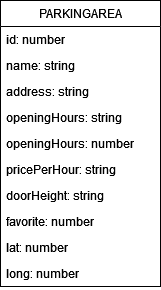
\includegraphics[width=0.2\linewidth]{table_parkingarea.png}
	\caption[Die Spalten und ihre Datentypen der Datenbanktabelle ,parkingarea'. Hier werden in \autoref{implementierung} alle Parkmöglichkeiten eingetragen.]
	{Die Spalten und ihre Datentypen der Datenbanktabelle ,parkingarea'. Hier werden in \autoref{implementierung} alle Parkmöglichkeiten eingetragen. (Quelle: Eigens erstellte Übersicht.)}
	\label{fig:parkingarea}
\end{figure}

Die zweite Datenbanktabelle erhielt den Namen ,parkingareadetails' und sollte mit den Daten der API gefüllt werden. Neben einer einzigartigen ID finden sich hier folgende Spalten: 
\begin{description}
	\item ID des jeweiligen Parkhauses \\ Um die Details der Parkmöglichkeiten denen der anderen Tabelle zuordnen zu können, wird zu jedem Datensatz die ID der Parkmöglichkeit gespeichert, zu der die Informationen gehören.
	\item Anzahl der Parkplätze \\ Die Anzahl der Gesamtheit aller Parkplätze der jeweiligen Parkmöglichkeit, unabhängig davon, ob diese belegt oder frei sind.
	\item Anzahl belegter Parkplätze \\ Die Anzahl der Parkplätze, die aktuell belegt sind.
	\item Anzahl freier Parkplätze \\ Die Anzahl der Parkplätze, auf denen noch geparkt werden kann.
	\item Trend \\ Der Trend gibt an, ob die Anzahl belegter Parkplätze steigt, sinkt oder gleich bleibt. Wenn beispielsweise viele Menschen auf einmal in die Parkmöglichkeit einfahren, so steigt der Trend. Der Trend kann die Werte 0 für ,gleichbleibend', 1 für ,steigend' oder -1 für ,fallend' annehmen.
	\item Status \\ Der Status, in welchem sich die Parkmöglichkeit befindet. Hierfür wird zwischen ,OK', ,Ersatzwerte', ,Manuell' oder ,Störung' unterschieden.
	\item Geschlossen \\ Dieser Wert zeigt an, ob die Parkmöglichkeit aktuell geöffnet oder geschlossen hat. Bei 0 ist die Parkmöglichkeit offen, bei 1 geschlossen.
	\item Datum und Uhrzeit der Daten \\ Um die aktuellsten Daten zu verwenden, müssen Datum und Uhrzeit, zu welcher die Daten erstellt sind, gespeichert werden.
\end{description}
In \autoref{fig:parkingareadetails} sieht man nochmals alle Spaltenbezeichnungen und die dazugehörigen Datentypen aufgelistet.

\begin{figure}[h]
	\centering
	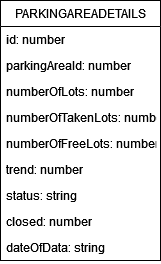
\includegraphics[width=0.2\linewidth]{table_parkingareadetails.png}
	\caption[Um die Daten der API verwenden zu können, wird eine Tabelle ,parkingareadetails' erstellt. Zu sehen sind hier die Spaltenbezeichnungen und die dazugehörigen Datentypen.]
	{Um die Daten der API verwenden zu können, wird eine Tabelle ,parkingareadetails' erstellt. Zu sehen sind hier die Spaltenbezeichnungen und die dazugehörigen Datentypen. (Quelle: Eigens erstellte Übersicht.)}
	\label{fig:parkingareadetails}
\end{figure}
  \chapter{Implementierung}
\label{implementierung}

In diesem Kapitel wird die Implementierung beschrieben. Zunächst werden die Komponenten und Klassen der Anwendung vorgestellt. Die gezeichneten Mockups unterscheiden sich nur minimal von der tatsächlichen Anwendung. Im Großen und Ganzen ist das Design aber gleich geblieben.

\section{Komponenten}
Die Komponenten bilden alle Funktionen der App, welche visuell auf der Benutzeroberfläche wahrgenommen werden. Neben der Anzeige der Elemente beinhalten sie aber dennoch auch Funktionalität, wie beispielsweise das Aufrufen von Methoden der Datenbank-Klasse ,DbConnectionService'. Alle Komponenten, mit Ausnahme der ,App', besitzen ein eigenes Interface. Dieses Interface beinhaltet alle Elemente, die als Properties in die Komponente hineingegeben werden und die jeweils dazugehörigen Typen. Properties können als Parameter an eine Komponente verstanden werden. Dies können neben Strings, Zahlenwerten oder boolschen Werten auch Funktionen oder andere Objekte sein.
\subsection{Komponente ,App'}
Die ,App'-Komponente kann sozusagen mit der ,main()'-Funktion anderer Programmiersprachen verglichen werden. Alles, was in dieser Funktion seinen Platz findet, findet sich auch in der Anwendung selbst wieder. Alle notwendigen Komponenten, die die Anwendung benötigt, werden hier eingefügt. 

Zu Beginn werden hier die Tabellen der Datenbank erstellt, sofern diese noch nicht existieren. Diese Komponente verwaltet die Daten. Die Informationen zu den Parkmöglichkeiten, die über die API abgerufen werden, werden zudem auch hier verwaltet. Durch den Hook ,useEffect' wird sichergestellt, dass die Daten nach einer bestimmten Zeit erneut abgefragt werden. Der Code hierfür kommt aus dem Internet und ist in \autoref{lst:useEffectApiData} zu sehen.

\begin{lstlisting}[caption={In diesem Hook werden nach der Zeit, welche sich hinter der Variable ,MINUTES\_MS' verbirgt, die Daten der API abgerufen, was über die Funktion in Zeile 3 geschieht. (Quelle: \cite{useIntervalCode})},captionpos=b, language=Java, label=lst:useEffectApiData]
	useEffect(() => {
		const intervalCall = setInterval(() => {
			dbConnectionService.getData();
		}, MINUTES_MS);
		return () => {
			clearInterval(intervalCall);
		};
	}, []);
\end{lstlisting}

Desweiteren gehehn auch die Daten des Eventhooks ,useGeofenceEvent', welcher in \autoref{geofenceEvent} erklärt wird, hier ein. Durch die Properties der anderen Komponenten werden die Daten dann an die richtigen Stellen gebracht. Wird ein Geofence betreten, so geschieht auch hier die Sprachausgabe. Der Button für das Ein- und Ausschalten des Tons befindet sich ebenfalls in der ,App'. Auch die Verwaltung des Tons liegt hier. Wird eine andere Ansicht geöffnet oder der Button zum Stummschalten der Sprachausgabe betätigt, so wird ein ,useEffect'-Hook getriggert, welcher die Sprachausgabe direkt beendet.

Neben verschiedenen ,set'- und ,get'-Funktionen, die für die Weitergabe von Daten zwischen Komponenten verantwortlich sind, befindet sich hier auch das Element, welches benötigt wird, um Toasts auszugeben. Alle Bestandteile in der ,<View>'-Komponente werden von ,<RootSiblingParent>' umrahmt, damit nachher an verschiedenen Stellen der Befehl aus \autoref{lst:toast} aufgerufen werden kann und somit in der Anwendung einen Toast anzeigt \cite{toastLibrary}.

\begin{lstlisting}[caption={Ein Beispiel des Aufrufs eines Toasts aus der Datei DbConnectionService. (Quelle: Eigene Implementierung)},captionpos=b, language=Java, label=lst:toast]
	Toast.show(errorMessages.noApiConnectionMessage, {
		duration: Toast.durations.LONG,
		position: Toast.positions.BOTTOM,
	});
\end{lstlisting}

\subsection{Komponente ,ParkingMap'}
Die wohl wichtigste Komponente der Anwendung ist die, welche die Karte beinhaltet. Diese findet sich hier. Zunächst wird beschrieben, welche Properties mitgeliedert werden. Hierzu ist es hilfreich, das zugehörige Interface ,IParkingMap' mit den Typen der Properties zu betrachten:
\begin{description}
	\item \textbf{handleParkingAreaId(id: number): void} \\ Hineingegeben wird eine Funktion ,handleParkingAreaId', welche nichts zurückgibt. Parameter ist hier ,id', was den Typ Nummer hat. Diese Funktion bringt die jeweilige ID der Parkmöglichkeit nach draußen in die ,App' und kann dort weiterverarbeitet werden.
	\item \textbf{handleParkingAreaDescription(parkingAreaDescription: boolean): void} \\ ,handleParkingAreaDescription' ist eine Funktion, welche nichts zurückgibt. Der Parameter dieser Funktion ist ein boolscher Wert namens ,parkingAreaDescription'. Diese Property hat in etwa denselben Nutzen, wie die eben beschriebene. Nur wird hier der ,App' mitgeteilt, ob die Beschreibung einer Parkmöglichkeit geöffnet werden soll oder nicht.
	\item \textbf{mapStyle: StyleProp<ViewStyle>} \\ Diese Property ist für das Design der ,ParkingMap' verantwortlich. Je nachdem, ob die Beschreibung der Parkmöglichkeit angezeigt wird oder nicht, ist die ,ParkingMap' größer oder kleiner.
\end{description}

Diese Komponete übernimmt die Anzeige der aktuellen Position des Nutzers und das Bilden der Geofences. Damit das funktioniert, benötigt man die Bibliothek Location von expo \cite{expoLocation}. Zur Nutzung von Geofences und der Anzeige der aktuellen Position wird die Erlaubnis des Nutzers für das GPS benötigt. Ohne diese Zustimmung wird dem Nutzer eine Meldung angezeigt, dass weder das Geofencing, noch die Anzeige der aktuellen Position funktionieren.

Um nun auch die Karte und die Marker an den Positionen der Parkhäuser anzeigen zu lassen, werden zusätzlich die Komponenten ,MapView' und ,Marker' der Bibliothek ,react-native-maps' benötigt. Je nach Gerät wird dann bei Android Google Maps und bei IOS Apple Maps verwendet. Um nun die Marker an den richtigen Stellen zu plazieren, wird die Liste aller Objekte der Parkmöglichkeiten mit der Funktion ,map()' durchgegangen und an jeder Stelle der Parkhäuser ein Marker gesetzt. Die Daten der Parkhäuser sind hier nicht aus der Datenbank, sondern aus dem Objekt-Array ,AllParkingAreas', welches in \autoref{AllParkingAreas} näher erklärt wird. Wird auf einen Marker geklickt, kommen die beiden Funktionen der Properties ins Spiel. Der Aufruf der Funktion ,handleParkingAreaId' mit der ID der angeklickten Parkmöglichkeit als Parameter lässt die ,App' wissen, welche Parkmöglichkeit angeklickt wurde. Wenn die Funktion ,handleParkingAreaDescription' mit dem Parameter ,true' aufgerufen wird, wird sichergestellt, dass sich dann immer die Beschreibung, welche in \autoref{fig:parkingAreaDescription} zu sehen ist, öffnet.

\begin{figure}[h!]
	\centering
	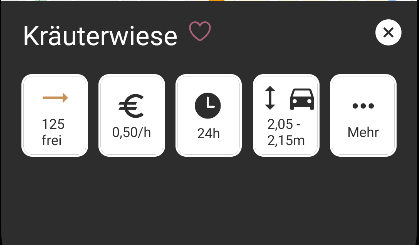
\includegraphics[width=0.45\linewidth]{parkingAreaDescription_component.png}
	\caption[Die Komponente ,ParkingAreaDescription', welche bei Klick auf einen Marker aufgerufen wird.]
	{Die Komponente ,ParkingAreaDescription', welche bei Klick auf einen Marker aufgerufen wird. (Quelle: Screenshot der erstellten Anwendung.)}
	\label{fig:parkingAreaDescription}
\end{figure}

\subsection{Komponente ,ParkingAreaDescription'}
\subsubsection{Komponente ,ParkingAreaDescriptionItemContainer'}
\subsection{Komponente ,ParkingAreaList'}
\subsubsection{Komponente ,ParkingAreaListItem'}
\subsection{Komponente ,ParkingAreaDetails'}
\subsubsection{Komponente ,ParkingAreaDetailsItem'}
\subsection{Komponente ,ParkingAreaListHeading'}
\section{Datenbankverbindung ,DbConnectionService'}
\section{Eventhook ,useGeofenceEvent'}
\label{geofenceEvent}
\section{Models}
\subsection{Interface ,IParkingArea'}
\subsection{Interface ,IParkingAreaDetails'}
\subsection{Interface ,IEventData'}
\section{Parkhausdaten ,AllParkingAreas'}
\label{AllParkingAreas}
\section{Weitere Hilfsmittel}
\subsection{Zentrale Verwaltung der Farben}
\subsection{Zentrale Verwaltung der Strings}
  \chapter{Starten der App}

 
  \phantomsection
  \addcontentsline{toc}{chapter}{Literaturverzeichnis}
  \begin{thebibliography}{10}
  	\bibitem{whyReactNative} Meta Platforms, Inc. (2023, Januar 05). React Native. Learn once, write anywhere. [online]. Verfügbar: \url{https://reactnative.dev/}.
  	
  	\bibitem{whyTypeScript} Microsoft. (2023, Januar 05). TypeScript is JavaScript with syntax for types. [online]. Verfügbar: \url{https://www.typescriptlang.org/}.
  	
  	\bibitem{whyExpo} Expo. (2023, Januar 05). What is Expo? An overview of Expo tools, features and services. [online]. Verfügbar: \url{https://docs.expo.dev/introduction/expo/}.
  	
  	\bibitem{colors} ColorSpace. (2023, Januar 05). Never waste Hours on finding the perfect Color Palette again! [online]. Verfügbar: \url{https://mycolor.space/?hex=%232E2D2D&sub=1}.
  	
  	\bibitem{icons} J. Arvidsson. (2023, Januar 05). react-native-vector-icons directory. [online]. Verfügbar: \url{https://oblador.github.io/react-native-vector-icons/}.
  	
  	\bibitem{locationIcon} Google (2023, Januar 15). Google Fonts. [online]. Verfügbar: \url{https://fonts.google.com/icons?selected=Material%20Symbols%20Outlined%3Alocation_on%3AFILL%400%3Bwght%40400%3BGRAD%400%3Bopsz%4048}
  	
	\bibitem{useIntervalCode} F. Hameed. (2023, Januar 05). How to call an API every minute for a Dashboard in REACT. For those looking for functional components. [online]. Verfügbar: \url{https://stackoverflow.com/questions/48601813/how-to-call-an-api-every-minute-for-a-dashboard-in-react}.
	
	\bibitem{toastLibrary} Horcrux. (2023, Januar 05). react-native-root-toast. [online]. Verfügbar: \url{https://github.com/magicismight/react-native-root-toast}.
	
	\bibitem{taskmanager} Expo. (2023, Januar 05). TaskManager. [online]. Verfügbar: \url{https://docs.expo.dev/versions/latest/sdk/task-manager/}.
	
	\bibitem{expoLocation} Expo. (2023, Januar 05). Location. [online]. Verfügbar: \url{https://docs.expo.dev/versions/v47.0.0/sdk/location/}.
	
	\bibitem{reactnativemaps} Airbnb. (2023, Januar 05). react-native-maps. [online]. Verfügbar: \url{https://github.com/react-native-maps/react-native-maps}.
	
	\bibitem{sqlite} Expo. (2023, Januar 05) examples. [online]. Verfügbar: \url{https://github.com/expo/examples/blob/master/with-sqlite/App.js#L14}.
	
	\bibitem{xmlParser} Autor unbekannt. (2023 Januar, 05). fast-xml-parser. [online]. Verfügbar: \url{https://www.npmjs.com/package/fast-xml-parser}.
	
	\bibitem{htmlEntities} Autor unbekannt. (2023 Januar, 05). html-entities. [online]. Verfügbar: \url{https://www.npmjs.com/package/html-entities}.
	
	\bibitem{tunneling} Expo. (2023, Januar 05). Expo CLI. [online]. Verfügbar: \url{https://docs.expo.dev/workflow/expo-cli/}
  \end{thebibliography}
  \newpage
  
  \phantomsection
  \addcontentsline{toc}{chapter}{Abbildungsverzeichnis}
  \listoffigures
  \newpage
  \addcontentsline{toc}{chapter}{Listingverzeichnis}
  \renewcommand{\lstlistlistingname}{Listingverzeichnis}
  \lstlistoflistings
  \appendix
\chapter{Anhang}
\label{mockups}

\end{document}    